\documentclass{article}

\usepackage{graphicx}
\usepackage{multimedia}
\usepackage{amssymb}

%\usepackage{algorithmic}
\usepackage{fancybox}
\usepackage{pseudocode}

\usepackage{pifont}
\usepackage{multirow}
\usepackage{slashbox}
\usepackage{pdfpages}
\usepackage{picture}

\usepackage{appendix}

\title{CS566 Parallel Processing \\ Assignment 04}
\author{Camillo Lugaresi and Cosmin Stroe \vspace{20pt} \\ Department of Computer Science \\
University of Illinois at Chicago}

\date{December 5, 2011}

\begin{document}

\maketitle
\newpage

\section{Algorithm Details and Formulations}




% \begin{figure}
% 	\centering
% 	\includegraphics[width=1.0\textwidth]{images/cannon-skew.pdf}
%     \label{fig:cannon-skew}
%     \caption{Explanation of the skew operation in Cannon's algorithm.}
% \end{figure}


\section{Results}


\section{Analysis and Lessons}

\clearpage

\appendix
%\includepdf[pages={-}]{code/pdf/cannon-c.pdf}
%\includepdf[pages=-]{code/pdf/cannon-h.pdf}
%\includepdf[pages=-]{code/pdf/dns-c.pdf}
%\includepdf[pages=-]{code/pdf/lu1d-c.pdf}
%\includepdf[pages=-]{code/pdf/lu2d-c.pdf}
%\includepdf[pages=-]{code/pdf/common-c.pdf}
%\includepdf[pages=-]{code/pdf/common-h.pdf}
%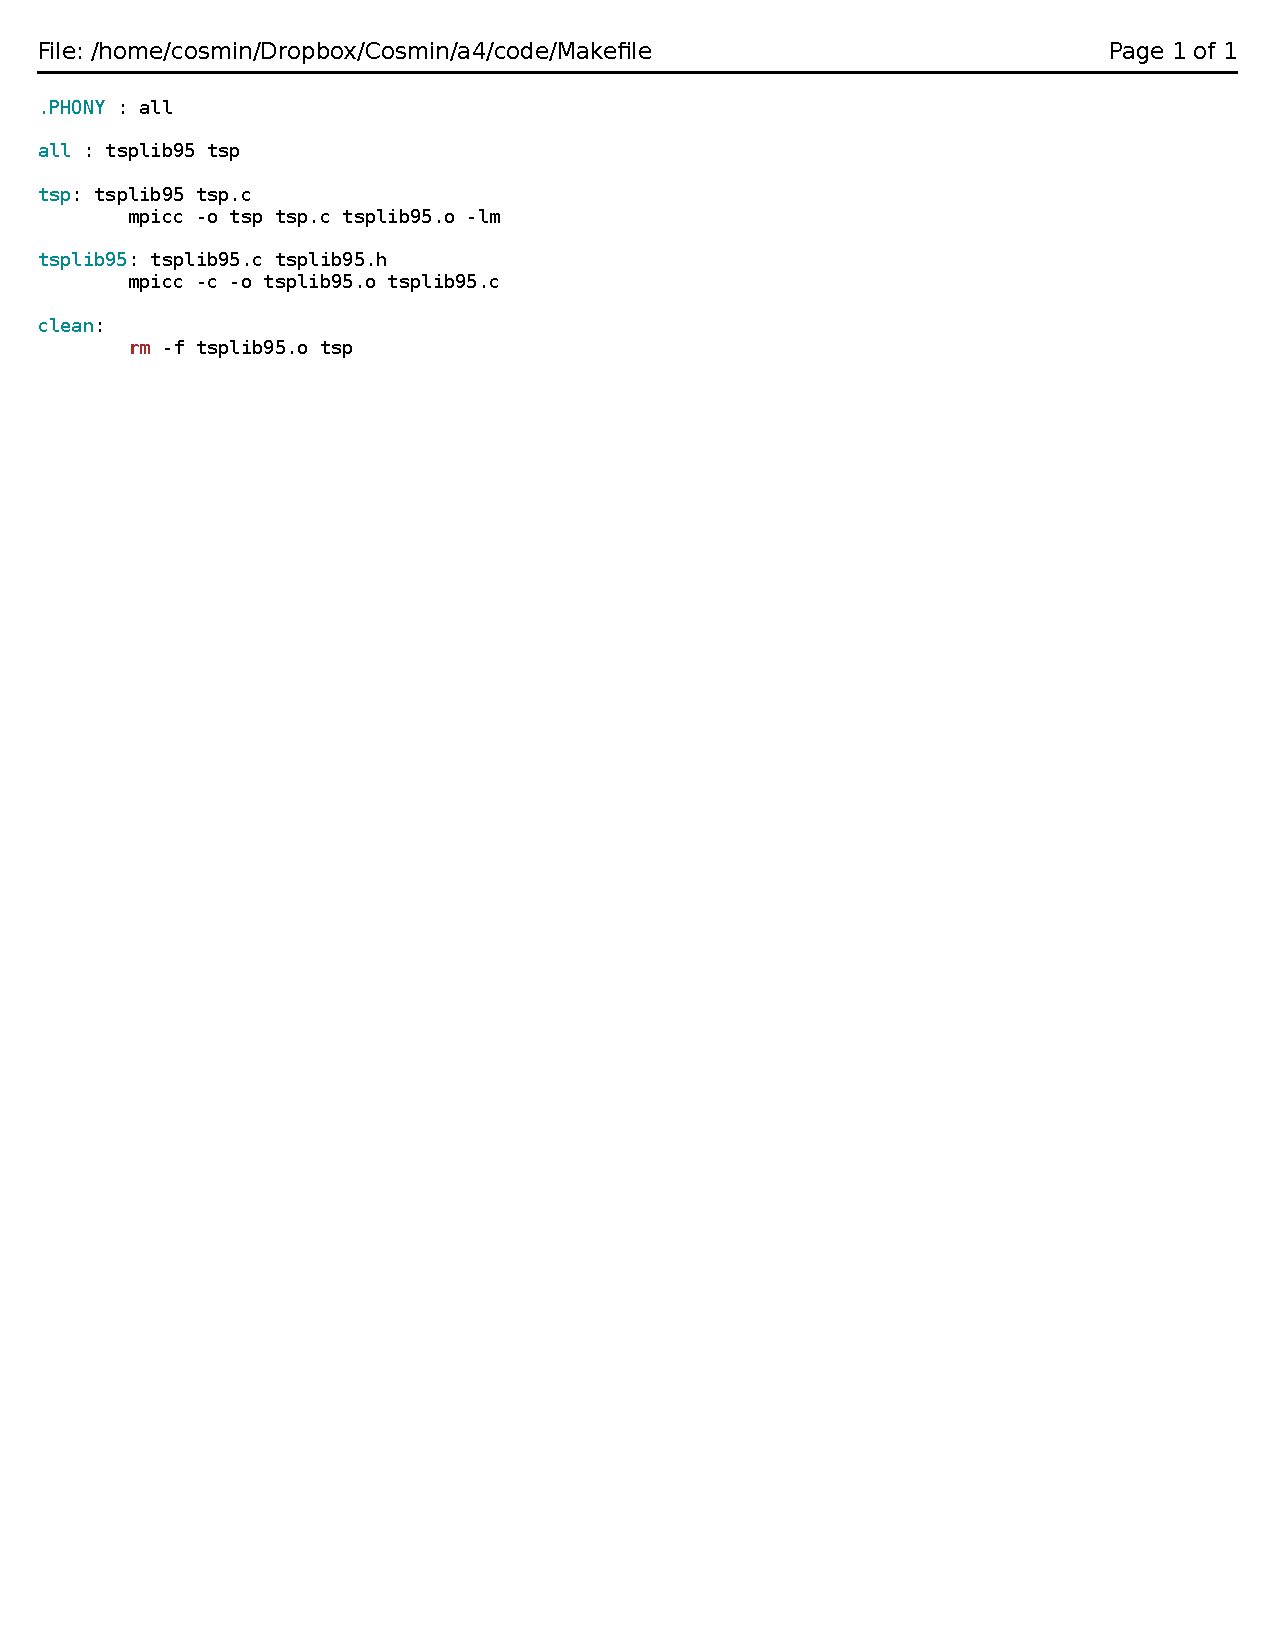
\includepdf[pages=-]{code/pdf/Makefile.pdf}

\end{document}
